
\subsection{Префиксный код}
\textbf{Префиксный код} - принцип однозначного кодирования, при котором для любых двух кодов $a$ и $b$, ни $a$ не является префиксом $b$, ни $b$ не является префиксом $a$.

Доказательство того, что декодирование в таком случае можно сделать однозначно настолько простое, что я оставлю его читателю. 

\subsection{Код Хаффмана}
\textbf{Код Хаффмана} - самый эффективный способ кодировать информацию в том случае, если каждый символ должен кодироваться целым числом бит и, если мы напрямую не пользуемся закономерностями данных, которые кодируем. 

Чтобы закодировать алфавит кодом Хаффмана мы должны иметь частоту появления каждого символа в тексте, который мы кодируем. Построим дерево Хаффмана на основе этих частот, каждый символ станет листом со своим весом, равным частоте появления этого символа в тексте, далее мы будем выполнять следующий алгоритм:
\begin{enumerate}
    \item Находим два элмента без родителя с наименьшим весом
    \item Создаем им родителя с весом, равным суммарному весу этих вершин
\end{enumerate}

Чтобы теперь задать бинарный код для каждого символа напишем на разных ребрах из одной вершины 0 и 1 и теперь, чтобы получить код для какого-то символа, нужно пройтись от корня до этого листа, и конкатенация цифр на ребрах и будет его кодом.
\begin{center}
  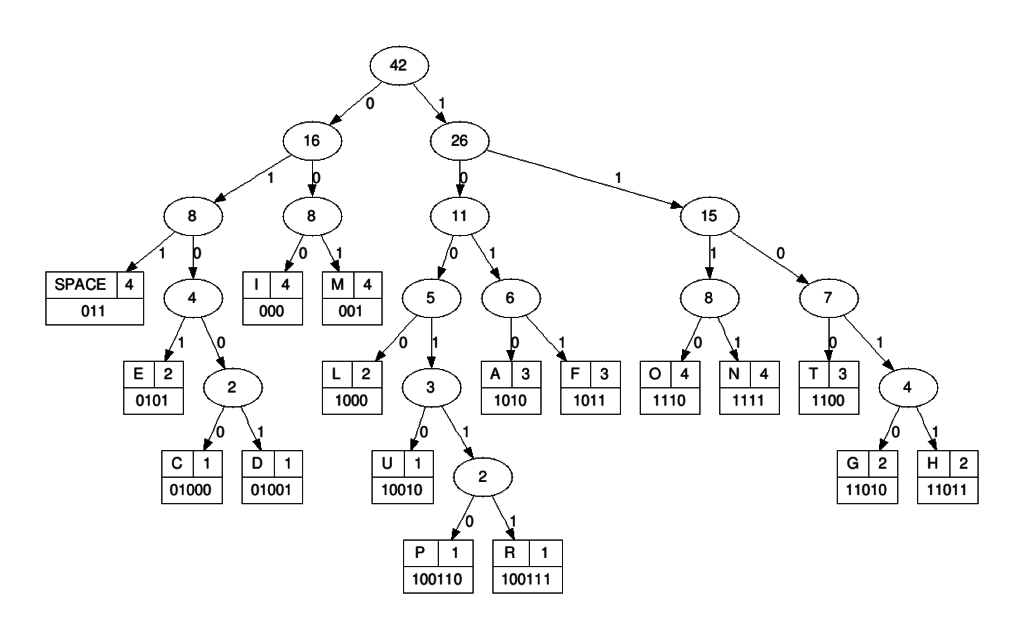
\includegraphics[height=9.1cm]{assets/huffman.png}
\end{center}

Докажем, что это кодирование оптимальнее любого другого. 

\textbf{Лемма} В дереве какого-то из оптимальных кодирований два символа с минимальным весом находятся на максимальной глубине и имеют общего родителя.
\textbf{Доказательство} Пусть это не так, посмотрим на 2 символа на максимальной глубине, имеющие общего родителя (такие обязательно найдутся, так как у нас нет вершин у которых всего 1 потомок, иначе их можно удалить). Эти вершины должны иметь максимальный вес, ведь если это не так, то мы можем поменять их с другими, которые имеют больший вес, а значит предыдущий код был не оптимальным. \textit{QED}

Заметим, что раз 2 вершины с максимальным весом находятся на максимальной глубине, то мы можем заменить их на их родителя, длина кода которого на 1 меньше, а вес тогда будет равен сумме их весов, получается мы уменьшаем общее количество символов на 1. Как раз так и строится дерево Хаффмана, а значит код Хаффмана является оптимальным.
\subsection{Неравенство Крафта-Макмиллана}
В общем случае неравенство Крафта-Макмиллана утверждает: 
Для того, чтобы для набора длин кодовых слов алфавита мощностью $r$: $l_1, l_2 \dots l_n$ существовал однозначно декодируемый код, необходимо и достаточно $$\sum\limits_{i=1}^n2^{-l_i}\leq 1$$
За доказательством \href{https://neerc.ifmo.ru/wiki/index.php?title=%D0%9D%D0%B5%D1%80%D0%B0%D0%B2%D0%B5%D0%BD%D1%81%D1%82%D0%B2%D0%BE_%D0%9C%D0%B0%D0%BA%D0%BC%D0%B8%D0%BB%D0%BB%D0%B0%D0%BD%D0%B0}{сюда}.
\